% GNUPLOT: LaTeX picture with Postscript
\begingroup
  \makeatletter
  \providecommand\rotatebox[2]{#2}%
  \@ifundefined{ifGPcolor}{%
    \newif\ifGPcolor
    \GPcolorfalse
  }{}%
  \@ifundefined{ifGPblacktext}{%
    \newif\ifGPblacktext
    \GPblacktexttrue
  }{}%
  % define a \g@addto@macro without @ in the name:
  \let\gplgaddtomacro\g@addto@macro
  % define empty templates for all commands taking text:
  \gdef\gplbacktext{}%
  \gdef\gplfronttext{}%
  \makeatother
  \ifGPblacktext
    % no textcolor at all
    \def\colorrgb#1{}%
    \def\colorgray#1{}%
  \else
    % gray or color?
    \ifGPcolor
      \def\colorrgb#1{\color[rgb]{#1}}%
      \def\colorgray#1{\color[gray]{#1}}%
      \expandafter\def\csname LTw\endcsname{\color{white}}%
      \expandafter\def\csname LTb\endcsname{\color{black}}%
      \expandafter\def\csname LTa\endcsname{\color{black}}%
      \expandafter\def\csname LT0\endcsname{\color[rgb]{1,0,0}}%
      \expandafter\def\csname LT1\endcsname{\color[rgb]{0,1,0}}%
      \expandafter\def\csname LT2\endcsname{\color[rgb]{0,0,1}}%
      \expandafter\def\csname LT3\endcsname{\color[rgb]{1,0,1}}%
      \expandafter\def\csname LT4\endcsname{\color[rgb]{0,1,1}}%
      \expandafter\def\csname LT5\endcsname{\color[rgb]{1,1,0}}%
      \expandafter\def\csname LT6\endcsname{\color[rgb]{0,0,0}}%
      \expandafter\def\csname LT7\endcsname{\color[rgb]{1,0.3,0}}%
      \expandafter\def\csname LT8\endcsname{\color[rgb]{0.5,0.5,0.5}}%
    \else
      % gray
      \def\colorrgb#1{\color{black}}%
      \def\colorgray#1{\color[gray]{#1}}%
      \expandafter\def\csname LTw\endcsname{\color{white}}%
      \expandafter\def\csname LTb\endcsname{\color{black}}%
      \expandafter\def\csname LTa\endcsname{\color{black}}%
      \expandafter\def\csname LT0\endcsname{\color{black}}%
      \expandafter\def\csname LT1\endcsname{\color{black}}%
      \expandafter\def\csname LT2\endcsname{\color{black}}%
      \expandafter\def\csname LT3\endcsname{\color{black}}%
      \expandafter\def\csname LT4\endcsname{\color{black}}%
      \expandafter\def\csname LT5\endcsname{\color{black}}%
      \expandafter\def\csname LT6\endcsname{\color{black}}%
      \expandafter\def\csname LT7\endcsname{\color{black}}%
      \expandafter\def\csname LT8\endcsname{\color{black}}%
    \fi
  \fi
  \setlength{\unitlength}{0.0500bp}%
  \begin{picture}(5040.00,1872.00)%
    \gplgaddtomacro\gplbacktext{%
      \csname LTb\endcsname%
      \put(372,468){\makebox(0,0)[r]{\strut{} 0}}%
      \put(372,772){\makebox(0,0)[r]{\strut{} 5}}%
      \put(372,1076){\makebox(0,0)[r]{\strut{} 10}}%
      \put(372,1379){\makebox(0,0)[r]{\strut{} 15}}%
      \put(372,1683){\makebox(0,0)[r]{\strut{} 20}}%
      \put(504,280){\makebox(0,0){\strut{} 500}}%
      \put(1310,280){\makebox(0,0){\strut{} 550}}%
      \put(2116,280){\makebox(0,0){\strut{} 600}}%
      \put(2923,280){\makebox(0,0){\strut{} 650}}%
      \put(3729,280){\makebox(0,0){\strut{} 700}}%
      \put(4535,280){\makebox(0,0){\strut{} 750}}%
      \put(0,1075){\rotatebox{-270}{\makebox(0,0){\strut{}count}}}%
      \put(2519,70){\makebox(0,0){\strut{}runtime (ms)}}%
      \put(2439,1562){\makebox(0,0)[l]{\strut{}100 consecutive runs of}}%
      \put(2439,1342){\makebox(0,0)[l]{\strut{}Safe Unrolled Stencil solver}}%
      \put(2439,1122){\makebox(0,0)[l]{\strut{}using 4 threads on 8 PEs}}%
    }%
    \gplgaddtomacro\gplfronttext{%
    }%
    \gplbacktext
    \put(0,0){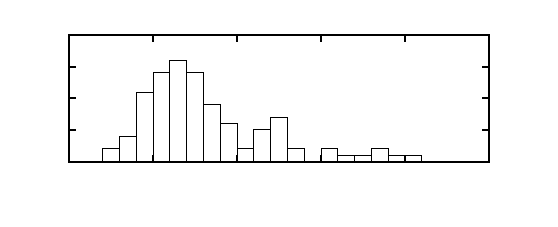
\includegraphics{data/laplace/tesla-repeat-qg-N4}}%
    \gplfronttext
  \end{picture}%
\endgroup
